\documentclass[12pt]{article}

% for special characters
\usepackage[utf8]{inputenc}
% for images
\usepackage{graphicx}
\graphicspath{{img/}}
% for source in images
\usepackage{floatrow}
% for urls
\usepackage{url}
% for references
\usepackage[sorting=none]{biblatex}
\addbibresource{references.bib}
% for multiple images
\usepackage{subfig}
% for automatic reference prefix
\usepackage{hyperref}
% for uppercase reference at the beginning of a sentence
\usepackage{cleveref}
% for good looking tables
\usepackage{booktabs}
% for lists with a), b), c)
\usepackage{enumitem}
% for equations with multicases
\usepackage{amsmath}

\begin{document}

\title{
\vspace{-2.0cm}

\includegraphics{zhaw}\\ 
\vspace{3cm}
Automated bone erosion scoring for rheumatoid arthritis with deep neural networks\\
{\Large Zurich University of Applied Sciences}}
\author{\begin{tabular}{rl}
  \textbf{Author:} & Janick Rohrbach \\
  \textbf{Supervisor:} & Dr. Oliver Dürr \\ & Prof. Dr. Beate Sick \\
  \textbf{Industrial Partner:} & Seantis GmbH \\
  \textbf{External Supervisor:} & Fabian Reinhard \\ & Dr. Tobias Reinhard \\
  \textbf{Date:} & December 22, 2017 \\
  \hspace{6.0cm} & \hspace{6.0cm}
\end{tabular}}
\date{}
\maketitle

\newpage

\section*{Declaration of originality\\ \large{Project Thesis at the School of Engineering}}
By submitting this project thesis, the undersigned student confirms that this thesis is his own work and was written without the help of a third party. \\
\\
The student declares that all sources in the text (including Internet pages) and appendices have been correctly disclosed. This means that there has been no plagiarism, i.e. no sections of the project thesis have been partially or wholly taken from other texts and represented as the student’s own work or included without being correctly referenced. \\
\\
Any misconduct will be dealt with according to paragraphs 39 and 40 of the General Academic Regulations for Bachelor’s and Master’s Degree courses at the Zurich University of Applied Sciences (Rahmenprüfungsordnung ZHAW (RPO)) and subject to the provisions for disciplinary action stipulated in the University regulations.\\
\vspace{3cm} \\
Zurich, December 22, 2017 \hspace{5cm} Janick Rohrbach

\newpage

\section*{Abstract}

Rheumatoid arthritis can cause irreversible damage to the joints. The severity of these bone erosions is scored by using x-ray images. This is usually done by a trained rheumatologist or radiologist and takes several minutes per patient.

This thesis shows a method to automatically score the joints in x-ray images with deep convolutional neural networks. We test a classification and a regression approach on x-ray images of joints from the left hand. In the classification task we predict the Ratingen-score on a discrete integer scale from 0 to 5. The model achieves normalized test and validation accuracies of XX \% and YY \% respectively. The regression model predicts the continuous percentage of bone erosion between 0 \% and 100 \% with a test and validation mean squared error of XXXX and YYYY respectively.

An automated scoring of bone erosion could help rheumatologists to spend less time with the scoring and have more time with the patient.

\newpage

\section*{Acknowledgements}
I would like to express my sincere thanks to my supervisors Beate Sick and Oliver Dürr who provided me with guidance and support during the writing of this thesis. 

I would also like to thank Fabian Reinhard and Tobias Reinhard (Seantis GmbH) for their valuable inputs. 

Further, I want to acknowledge the SCQM foundation which made this thesis possible by providing the comprehensive dataset. A list of rheumatology offices and hospitals that are contributing to the SCQM registries can be found on www.scqm.ch/institutions. The SCQM is financially supported by pharmaceutical industries and donors. A list of financial supporters can be found on www.scqm.ch/sponsors.

\newpage

\tableofcontents

\newpage

\section{Introduction}

This thesis shows a method for the automated scoring of x-ray images of patients with rheumatoid arthritis.

\subsection{Background}

Rheumatoid arthritis is an autoimmune disease. Which means that the disease is caused by a malfunctioning immune system. The immune system attacks healthy tissue instead of bacteria and viruses. This causes inflammation in the joints. Irreversible damage to the bone in the joint can occur, if the inflammation lasts for a long time. \cite{rheuma} Rheumatoid arthritis is incurable, merely the symptoms can be treated.

Today, the severity of the bone erosion is assessed by a trained rheumatologist by using x-ray images of hand and feet. This process takes several minutes per patient. This thesis shows, how recent advances in computer vision make it possible to automate this task. This leads to time savings which in return help the rheumatologist to spend more time with the patient.

The Swiss Clinical Quality Management in Rheumatic Diseases (SCQM) Foundation runs a national registry of inflammatory rheumatic diseases. \cite{scqm_about} They have collected anonymized patient data for over 10 years and provide the x-ray images used for this analysis.

Seantis GmbH, the industrial partner for this thesis, is a Swiss company that develops data driven web applications for medical research, pubic administration and aviation. \cite{seantis_about} For their customer SCQM they want to automate the bone erosion assessment. They already have a working algorithm, which detects the body part shown in the x-ray image. A second algorithm detects the joints in the image and extracts them as single images. These images are then used together with the bone erosion scores to train our model.

% Stand der Technik: Bisherige Lösungen des Problems und deren Grenzen 
% (Nennt kurz den Industriepartner und/oder weitere Kooperationspartner und dessen/deren Interesse am Thema Fragestellung) 

\subsection{Related literature}

% Nennt bestehende Arbeiten/Literatur zum Thema Literaturrecherche

There are several applications where convolutional neural networks are used in medical research.

A recent paper from Tajbakhsh et al. \cite{tajbakhsh_2017} investigated whether fine-tuning a pre-trained CNN is better than training a CNN from scratch when applied to medical images. They find that pre-trained networks with fine-tuning always outperformed or at least performed as well as CNNs trained from scratch. They further recommend a layer-wise fine tuning which seems to outperform shallow and deep tuning.

A study by Paul et al. \cite{paul_2017} tried to classify osteoporosis by considering x-ray images of the bone. This task proved to be very difficult as the x-ray images from healthy patients look very similar to the ones of patients with the disease. By using a transfer learning approach they achieved a validation accuracy of 44.82 \%.

Zhou et al. \cite{zhou_2002} used a two-level ensemble of neural networks to identify lung cancer cells on x-ray images of the chest. The first-level ensemble classifies whether a cell is a cancer cell or not by using full voting. The second-level ensemble is used only on cells classified by the first-level as cancer cells. It differentiates between different cancer classes as well as a non-cancer class. This ensemble works with plurality voting. The authors state that this method achieves a high accuracy and a low rate of false negatives.

A report from Chen \cite{chen_2016} showed the application of convolutional neural networks on x-ray images of hands to predict the developmental bone age. He achieves a top one and two accuracy of 46 \% and 70 \% respectively. This result is close to previously used methods which use manual segmentation and handcrafted features.

In a degree project Hensman and Masko \cite{hensman_2015} looked at the impact of imbalanced training data for CNNs. They find, that heavy imbalances have a strong impact on the performance and suggest oversampling of minority classes to improve the performance of the network.

\subsection{Aim and scope of this thesis}

The aim of this thesis is to predict bone erosion scores from x-ray images. We further examine how the bone erosion and the disease activity are correlated.

The work is based on images of the left hand only. There also exist images of right hands as well as images of left and right feet. But at this point in time, only the joints of left hands have been extracted from the images. It is assumed that the model will perform similar on the joints of the right hand. By fine-tuning the model on the images of joints from feet it should also perform well for those images.

\newpage

\section{Theory}
\label{sec:theory}

\subsection{Finger joints}
\label{subsec:joints}

\autoref{fig:joints} shows an x-ray image of a left hand similar to the images received from the SCQM foundation. The five proximal interphalangeal (PIP) joints and the five carpometacarpal (MCP) joints are shown with blue bounding boxes. These are the joints, that are most affected by rheumatoid arthritis. The wrist joint is also affected, but we limited our analysis to the five PIP joints and the five MCP joints. Each of these joints is assessed with a score by a trained rheumatologist or radiologist. The scoring method is described in the next section.

\begin{figure}[ht]
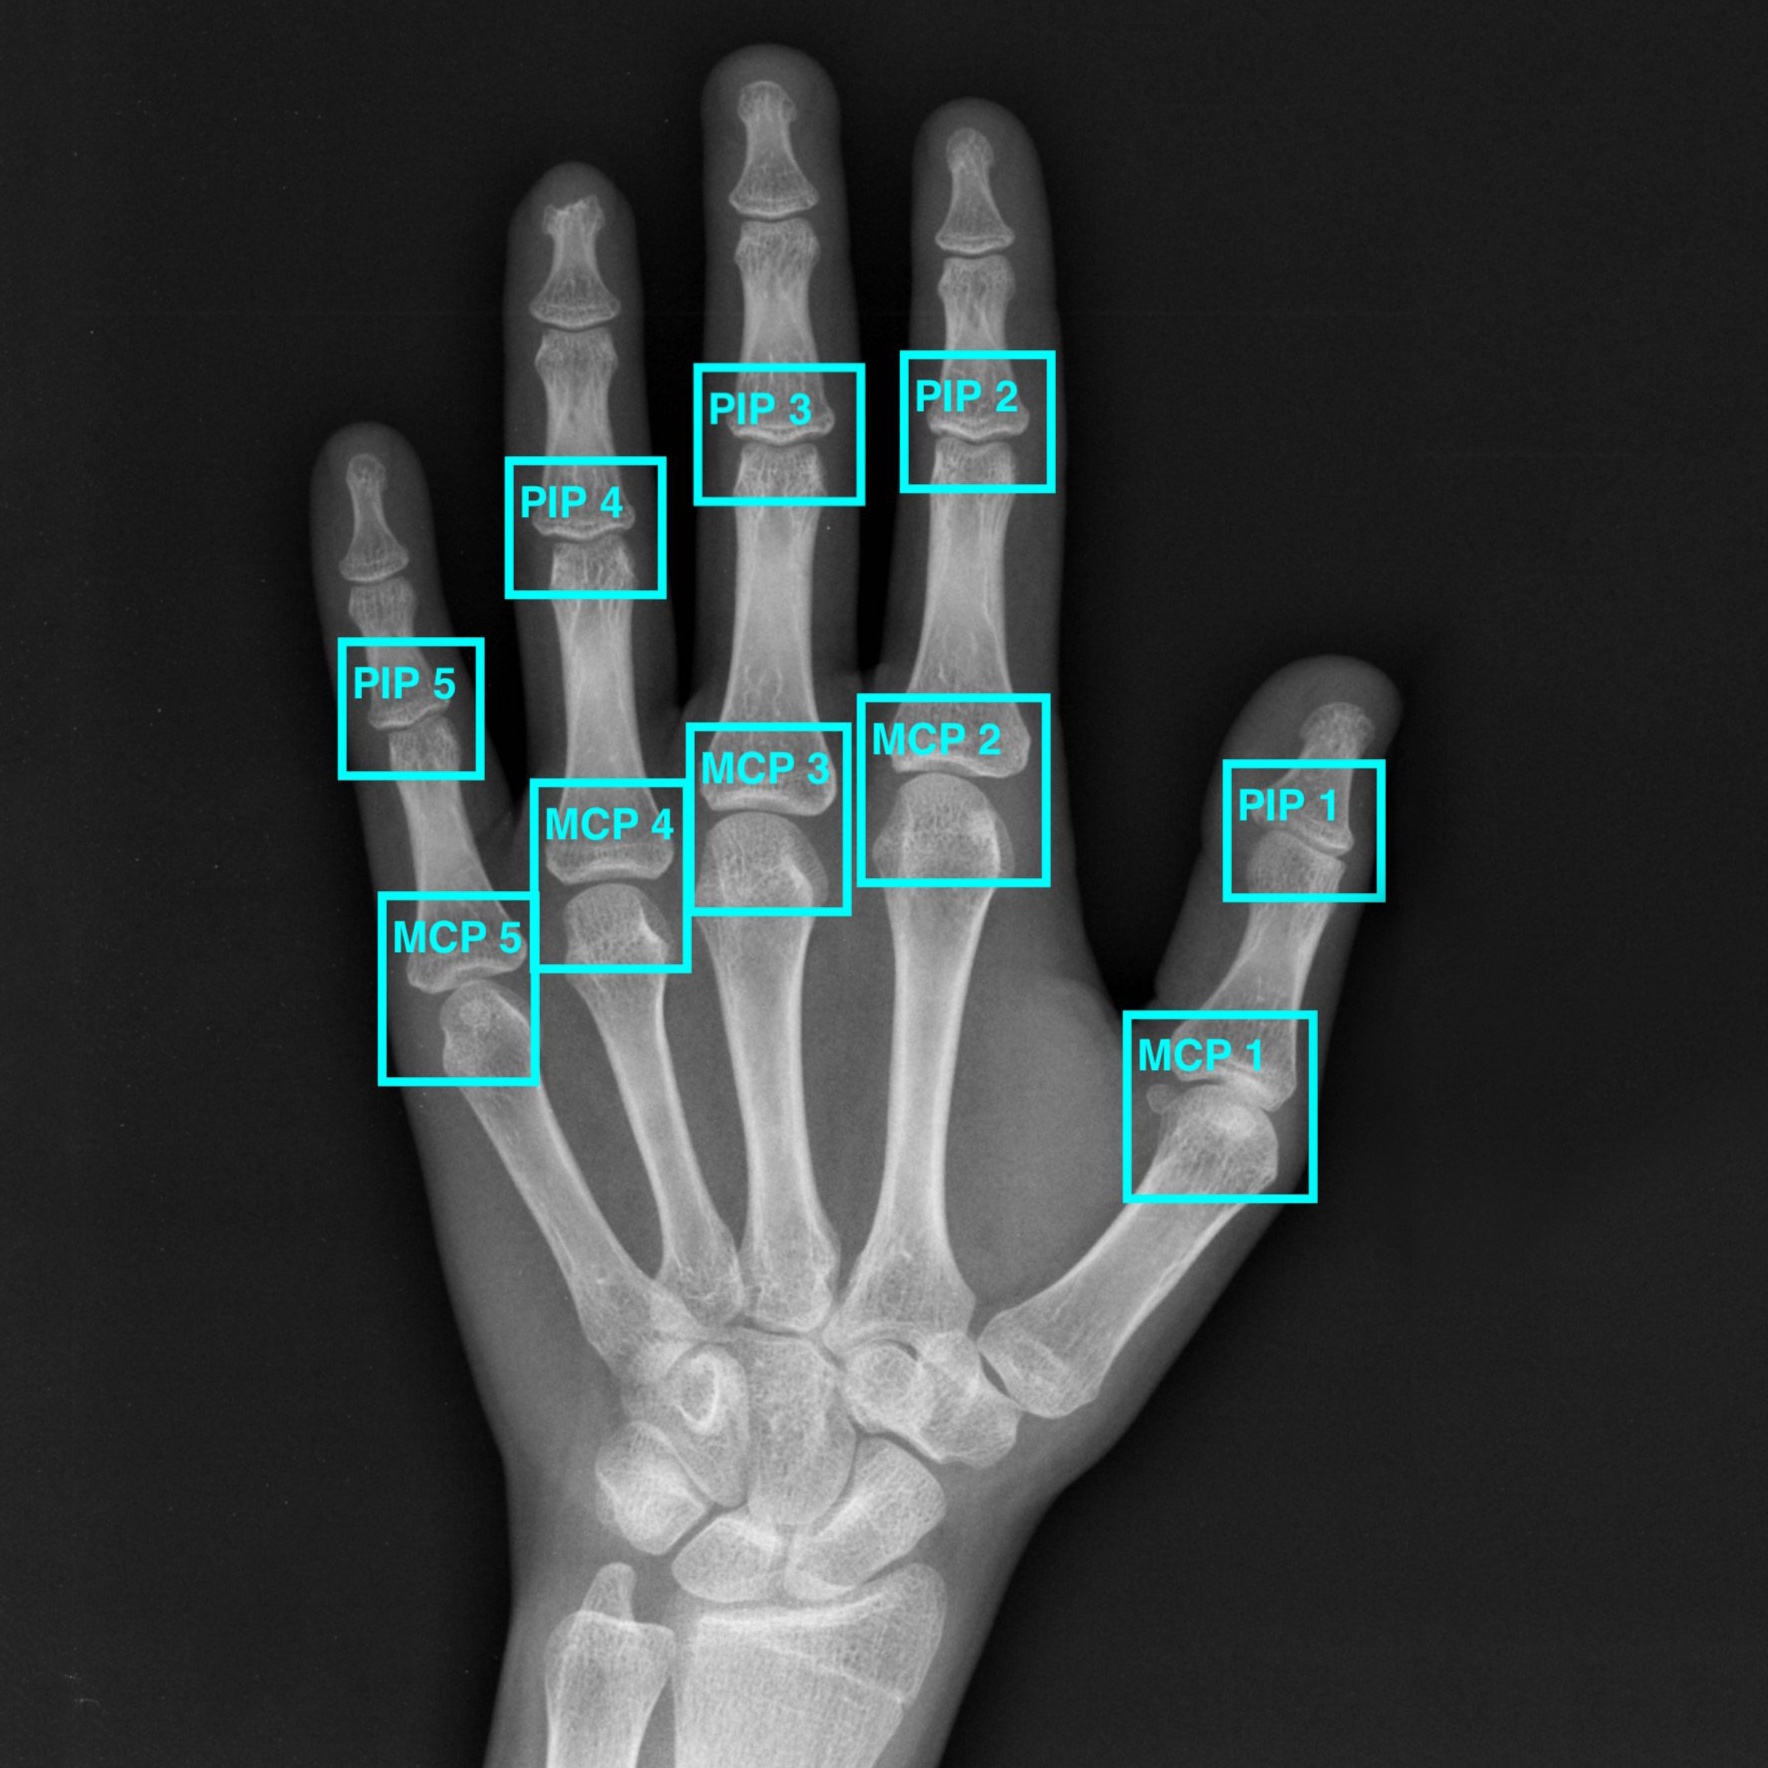
\includegraphics[width=10cm]{joints}	
\caption{Proximal interphalangeal (PIP) joints and carpometacarpal  (MCP) joints.}
\floatfoot{Original image by Nevit Dilmen (CC BY-SA) \url{https://commons.wikimedia.org/wiki/File:Medical\_X\-Ray\_imaging\_OPC06\_nevit.jpg}}
\label{fig:joints}
\end{figure}

\subsection{Ratingen-score}
\label{subsec:ratingen}

The most important criteria for the effectiveness of a treatment is the influence on the radiological progression. To quantify the irreversible bone erosion in the joint, several scoring methods were developed. The score used in this thesis is called Ratingen-score, it estimates the percentage of eroded joint surface. \cite{rau_2007}. The labels of our data lie within 0 and 100 and correspond to the percentage of joint surface erosion. These values can easily be converted to Ratingen-Scores according to \autoref{tab:ratingen}.


\begin{table}[ht]
\centering
\caption{Disease stages of Ratingen-score \cite{rau_2007} }
\label{tab:ratingen}
\begin{tabular}{@{}ll@{}}
\toprule
Stage & Description                                                          \\ \midrule
0     & Normal joint                                                         \\
1     & One or more erosions, less than 20 \% of the joint surface is eroded \\
2     & 21 \% - 40 \% of the joint surface is eroded                         \\
3     & 41 \% - 60 \% of the joint surface is eroded                         \\
4     & 61 \% - 80 \% of the joint surface is eroded                         \\
5     & More than 80 \% of the joint surface is eroded                       \\ \bottomrule
\end{tabular}
\end{table}

\subsection{Rau-score}
\label{subsec:rau}

This score is an overall score, which is calculated from the individual Ratingen-scores. The sum of the Ratingen-scores for all 32 joints (5 PIP, 5 MCP and 1 wrist joint per hand and 5 joints per foot) is multiplied by 38 and divided by the number of scored joints.

\subsection{Disease activity score (DAS28)}
\label{subsec:das}

The disease activity score (DAS28) measures the disease activity for the following 28 joints. 5 PIP, 5 MCP and 1 wrist joint per hand plus elbow, shoulder and knee joints \cite{runmc}. The score is derived from the following four measurements.

\begin{enumerate}[label=(\alph*)]
\item $n_s =$ Number of swollen joints
\item $n_t =$ Number of tender joints
\item $ESR$ in mm/hr or $CRP$ in mg/L $=$ Blood markers of inflammation (either the erythrocyte sedimentation rate (ESR) or C reactive protein (CRP))
\item $g_h$ in mm $=$ Patients global assessment of disease activity on a 100 mm long scale from very good (0 mm) to very bad (100 mm).
\end{enumerate}

The DAS28 score is then calculated as follows. \cite{runmc_formula}
\\
\\
$DAS28_{ESR} = 0.56 * \sqrt{n_t} + 0.28 * \sqrt{n_s} + 0.7 * \ln{(ESR)} + 0.014 * g_h$
\\
\\
$DAS28_{CRP} = 0.56 * \sqrt{n_t} + 0.28 * \sqrt{n_s} + 0.36 * \ln{(CRP + 1)} + 0.014 * g_h + 0.96$
\\
\\
\begin{tabular}{@{}llll}
$DAS28$ & $>$ & $5.2 =$ & high disease activity \\
$DAS28$ & $<$ & $3.2 =$ & low disease activity \\
$DAS28$ & $<$ & $2.6 =$ & remission
\end{tabular}

\subsection{Artificial neural networks}
\label{subsec:ann}
This section offers a very brief introduction to artificial neural networks. A more in-depth explanation can be found in Andrey Karpathy's course notes for the Stanford class CS231n. \cite{karpathy}

The structure of an Artificial neural network (ANN) is inspired by the human brain. A brain consists of approximately 100 billion neurons which form an interconnected network. The neurons can communicate with each other by transmitting electrical potential. If the potential in a neuron reaches a certain threshold, it fires and transmits the potential to connected neurons. \cite{kruse_2016}

An ANN is a very simplified model of this biological process. A single neuron can be described by the following equation. $$f\left(\sum_{i}w_i*x_i+b\right)$$ Where $x_i$ are the inputs, $w_i$ are the weights and $b$ is a bias term. The activation function $f$ models the firing of the neuron.

These single neurons can then be combined to networks. The most simple network is the fully connected neural network described in the following section.

\subsubsection{Fully connected neural networks}
\label{subsubsec:fcnn}
A fully connected neural network (FCNN) has an input layer, arbitrarily many hidden layers and one output layer. The neurons of each layer are connected to every neuron of the next layer. The data  can only flow in one direction, from the input layer towards the output layer. \autoref{fig:fcnn} shows a possible structure for a FCNN.

\begin{figure}[ht]
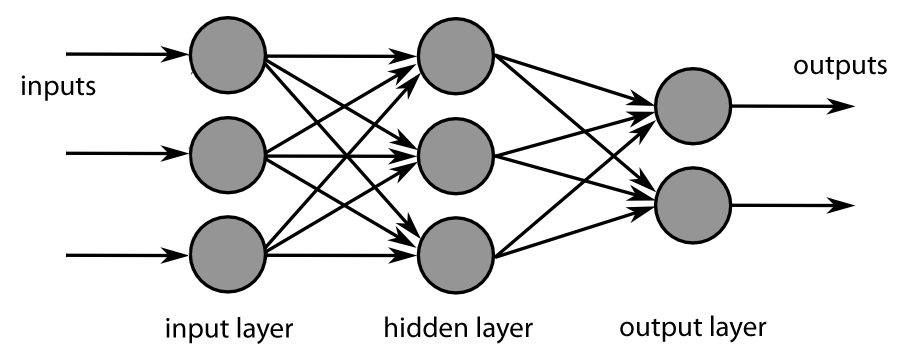
\includegraphics[width=10cm]{ffnn}	
\caption{Feed forward neural network with one hidden layer.}
\floatfoot{Image by Chrislb (CC BY-SA) \url{https://commons.wikimedia.org/wiki/File:MultiLayerNeuralNetworkBigger_english.png}}
\label{fig:fcnn}
\end{figure}

The number of neurons per layer specifies the width of the neural network, whereas the number of hidden layers specifies the depth of a neural network. A neural network with many hidden layers is called a deep neural network.

For supervised learning the weights and biases of this network can be trained by using back-propagation. The input is fed through the network with randomly initialized parameters. The output is then compared to the true values by using a loss-function. The loss is then back-propagated through the network to adjust the parameters. With every training step, this process is repeated and the loss decreases. This process is also called learning. And for deep neural networks we speak of deep learning.

A special type of the FFNN, used for image recognition, is the convolutional neural network, which is described in the next section.

\subsubsection{Convolutional neural networks}
\label{subsubsec:cnn}
Convolutional neural networks (CNNs) take an image as an input. The image can be seen as a 3-dimensional matrix, where the third dimension includes the different color channels. Instead of fully connected layers, convolutional layers are used. Convolutions work as filters that detect different features in the image. These filters usually have a small size (e.g. 3x3) and are moved over the image. \autoref{fig:cnn} shows a possible architecture of a CNN with multiple convolutional layers and a fully connected layer at the end.

\begin{figure}[ht]
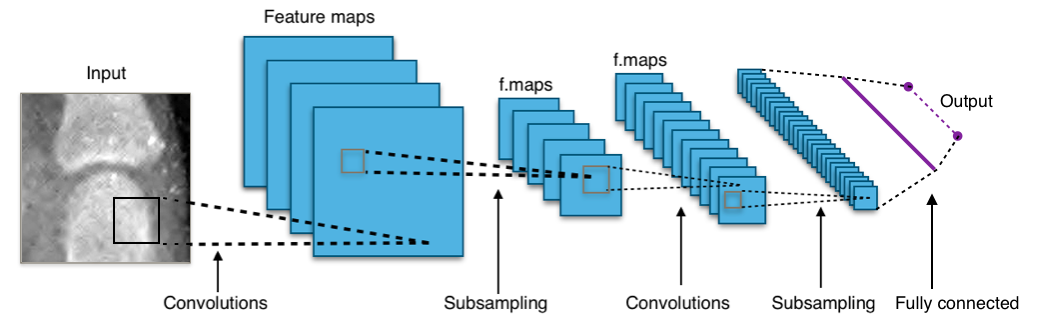
\includegraphics[width=10cm]{cnn}	
\caption{Structure of a convolutional neural network.}
\floatfoot{Original  image by Aphex34 (CC BY-SA) \url{https://commons.wikimedia.org/wiki/File:Typical_cnn.png}}
\label{fig:cnn}
\end{figure}

In contrast to classical machine learning we don't need to extract any features beforehand. The hidden layers of the deep convolutional neural network will do the feature extraction automatically.

\newpage
\section{Data}
\label{sec:data}

The received data consists of jpg images of the joints and two csv datasets. The main dataset includes the following columns.

\begin{table}[ht]
\centering
\caption{Columns of main dataset}
\label{tab:main_dataset}
\begin{tabular}{@{}ll@{}}
\toprule
Column name   & Description                                           \\ \midrule
id\_x         & Unique observation id                                 \\
patient\_id   & Unique patient id                                     \\
date\_x       & Date of the consultation                              \\
date\_y       & Date on which the joints were scored                  \\
sop\_iuid     & Unique x-ray image id                                 \\
body\_part    & Left/right hand/foot or both hands/feet               \\
hand\_left\_x & Percentage of bone erosion for joint x                \\
rau\_score    & Overall Rau-score described in \autoref{subsec:rau} \\ \bottomrule
\end{tabular}
\end{table}

This is the dataset where the percentages of bone erosion for the joints of the left hand were extracted. The corresponding x-ray image can be found by using the sop\_iuid.

The secondary dataset contains additional scores which only exist for some of the patients and some consultations.

\begin{table}[ht]
\centering
\caption{Columns of secondary dataset}
\label{tab:sec_dataset}
\begin{tabular}{@{}ll@{}}
\toprule
Column name   & Description                                           \\ \midrule
patient\_id   & Unique patient id                                     \\
date       & Date of the consultation                              \\
physician\_global\_disease\_activity       & Medical global assessment of disease activity                \\
global\_patient\_estimate\_disease\_activity     & Patient estimate of disease activity   \\
das28bsr\_score    & DAS28BSR as described in \autoref{subsec:das}             \\
das283crp\_score & DAS28ERP as described in \autoref{subsec:das} \\ \bottomrule
\end{tabular}
\end{table}

The two datasets can be merged on patient\_id and date/date\_x.


\subsection{Data preparation}
\label{subsec:data_prep}

The data preparation step brings the jpg images into a suitable format that can be used as an input for the CNN. 

The original images have values between 0 and 255. We divided the data by 255 in order to have values in the range of [0,1].

The data was randomly split into a training set (70 \% of the data), a test set (20 \% of the data) and a validation set (10 \% of the data). It was split such that all images of the same patient are in the same set.

The images of the joints have varying exposure. Some images are very dark while others are very bright. It was therefore considered to apply a histogram equalization, which is a linear transformation that maps the lightest pixel to 255 and the darkest pixel to 1. However, this transformation did not improve the accuracy of the model and was not used for the final model.

The bone erosion scores of the labeled joints are highly imbalanced. As seen in \autoref{fig:imbalance} most of the joints are healthy and received a score of 0. There are quite a few observations with little bone erosion with scores between 0 and 25. There are very little observations with scores higher than 25. Only the fully eroded joints (score = 100) seem to be a bit more frequent.

\begin{figure}[ht]
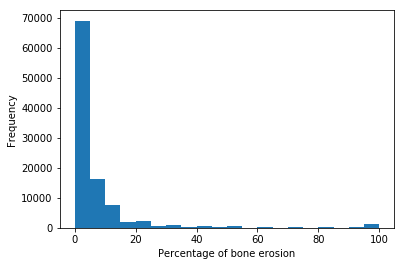
\includegraphics[width=10cm]{imbalance}	
\caption{Histogram of the bone erosion scores}
\label{fig:imbalance}
\end{figure}

When training the CNN, it minimizes the overall loss-function. For imbalanced data the CNN performs bad for the underrepresented part of the data. In this case, the model would be bad predictor for high scores. In order to make the model a good predictor for all cases, we tried weighting the loss function as well as oversampling the underrepresented classes.



\newpage
\section{Methods and results}
\label{sec:methods&results}

In order to predict the bone erosion scores, different models were evaluated. This section describes the different steps in the evaluation process. It shows a classification model which predicts the Ratingen-score and a regression model which predicts the percentage of bone erosion.

\subsection{Software and infrastructure}
The models were built in Python 3.5 \cite{python} with the package Tensorflow 1.4 \cite{tensorflow} using the high level API Keras \cite{keras}. For general machine learning the package Scikit-learn \cite{scikit-learn} was used. The package Matplotlib \cite{matplotlib} was used to produce figures. In addition, the programming language R \cite{r} was used for further analysis of the results and for producing figures.

For the training of the models a Nvidia Titan X (Pascal) graphics card was used.

\subsection{Base models}

We decided to create a classification as well as a regression model. The architecture of both models is similar and is inspired by the VGG16 net. It consists of 6 blocks of two convolutional layers of the size 3x3 followed by a max pooling layer. The number of filters per convolutional layer is increasing with every second block, whereas the size of the layers is decreasing due to the max pooling layers. Every convolutional layer uses batch normalization before the ReLu activation function.

This first part is identical for both models. We then flatten the output of the last convolution block and use two dense layers with batch normalization, ReLu activation and dropout. Only the number of neurons in the dense layers is different between the two models. The output layer however is different between the two models and described in the next two sections.

\subsubsection{Classification model}
\label{subsubsec:clas}

The classification model directly predicts the Ratingen-score. The output layer has 6 neurons according to the 6 Ratingen classes (0-5). The Softmax activation function is then used to predict the probabilities for each class. The architecture of this CNN is shown in \autoref{fig:cnn_cla}.

\begin{figure}[ht]
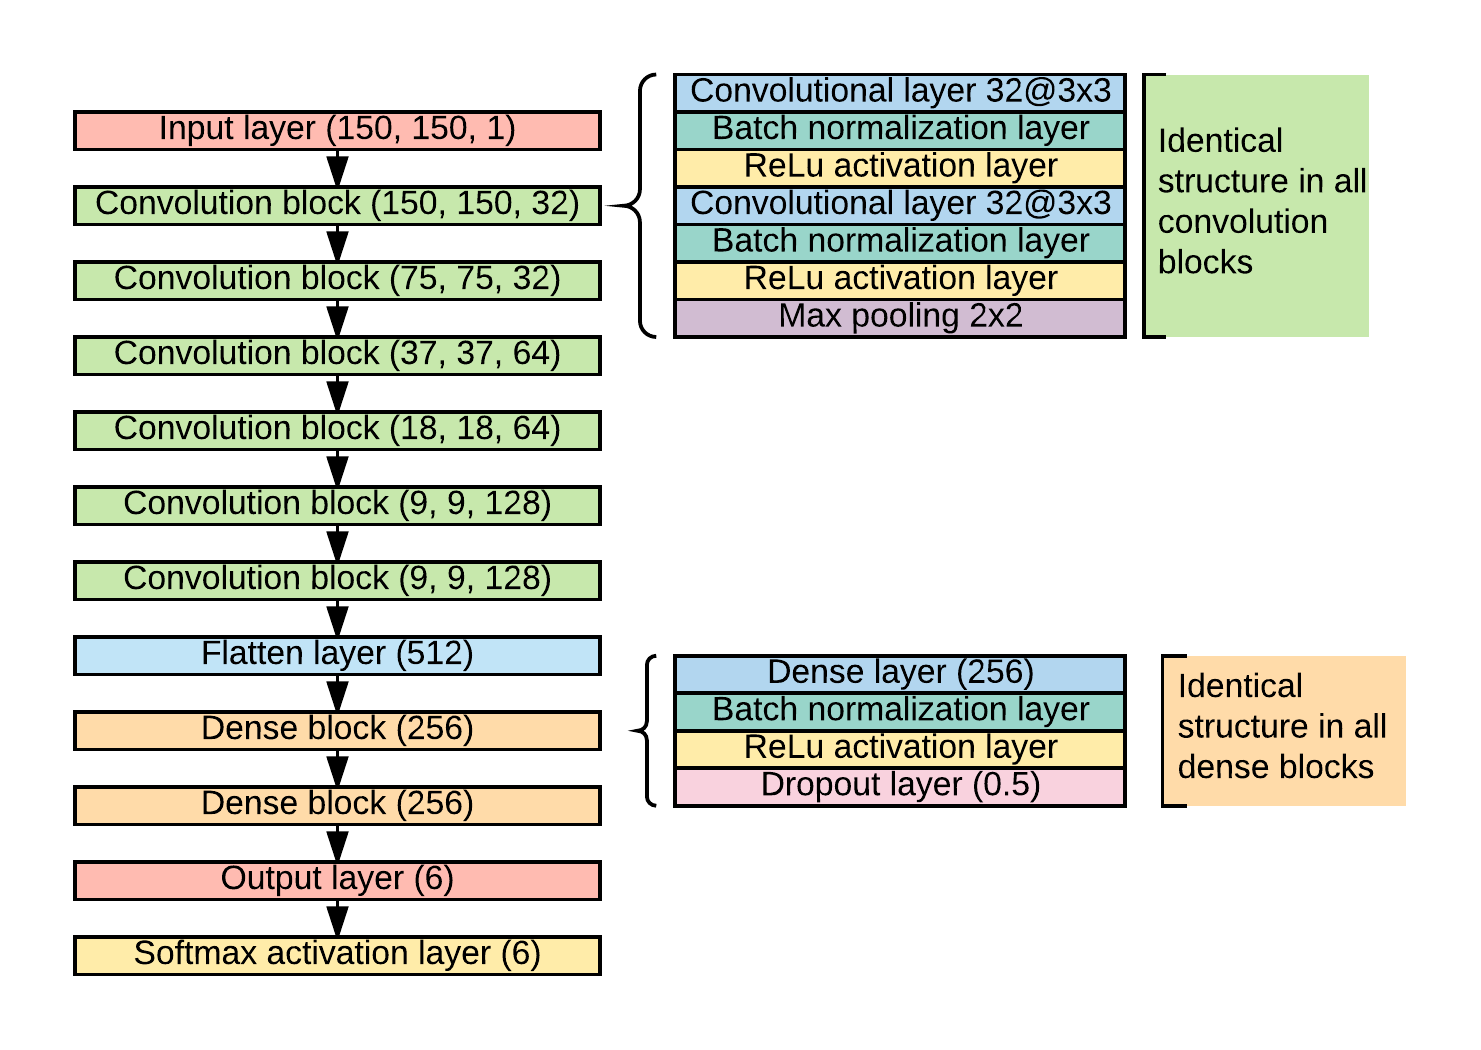
\includegraphics[width=10cm]{cnn_classification}	
\caption{Architecture of the CNN for classification}
\label{fig:cnn_cla}
\end{figure}

The model is trained for 25 epochs with the ADAM optimizer and a learning rate of 0.001. Categorical loss entropy is used as the loss function. The images are fed through the model in batches of 100 images at a time.

As described in \autoref{subsec:data_prep} we tried different approaches to handle the imbalanced data. 

\begin{enumerate}[label=(\alph*)]
\item The first model is trained on the original data and is used as a basis to compare the results of the other models.
\item For the second model we oversampled the underrepresented classes in order to have roughly the same number of images per class. The oversampled images are augmentations of the original data. Random rotations of up to 25 degrees, shearings of up to 0.1 radians and and zooms of up to 10 \% were used.
\item The third model used the same data as the first model, but the loss function was weighted with class weights. The class weights where chosen such that the class weight multiplied by the number of observation in that class equals to the same value for all classes.
\end{enumerate}

Model b) was trained for the full 25 epochs, whereas the other two models started overfitting and had to be stopped early after 9 epochs. \autoref{fig:confusion} shows the normalized confusion matrices for the test dataset for the three models.

\begin{figure}[ht]
\begin{tabular}{ccc}
\subfloat[Original data]{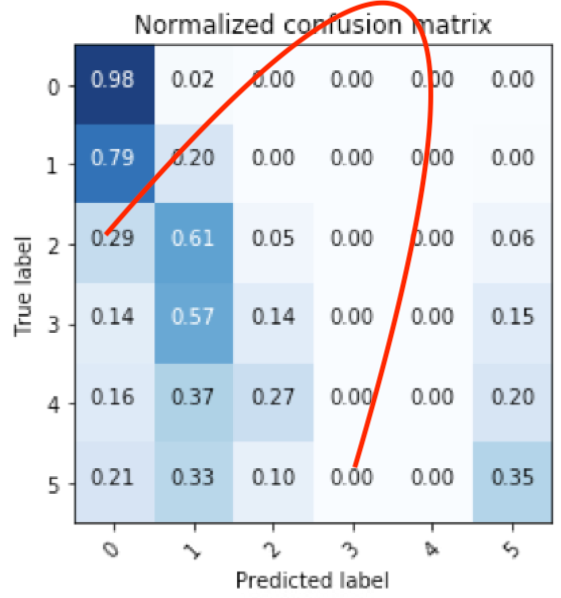
\includegraphics[width = 1.5in]{classification_original}} &
\subfloat[Oversampled]{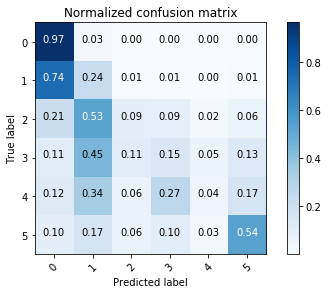
\includegraphics[width = 1.5in]{classification_oversampled}} &
\subfloat[Weights]{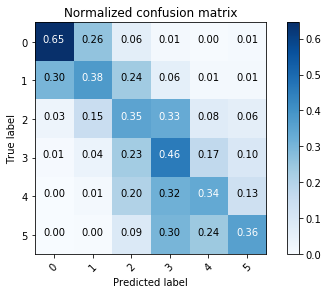
\includegraphics[width = 1.5in]{classification_weights}}
\end{tabular}
\caption{Normalized confusion matrices for the predictions of the classifcation models.}
\label{fig:confusion}
\end{figure}

The evaluation metrics for the three models can be seen in \autoref{tab:metrics_cla}. It turned out that the accuracy is not a suitable metric. Model a) has the highest accuracy but makes a lot of misclassifications in the under-represented classes. Whereas the accuracy of model c) is the lowest, but the accuracy for the underrepresented classes is much better.

Therefore, we decided to use the class normalized accuracy as our evaluation metric. It is the mean of the six class accuracies. It describes much better, whether our model is a good predictor for all classes.

As a second metric, we calculated the class normalized accuracy for predictions that are in the right class or no more than one class above or below the correct class. This metric takes into account, that a misclassification by 1 is far less severe than a misclassification by 5.

\begin{table}[ht]
\centering
\caption{Evaluation metrics for classification.}
\label{tab:metrics_cla}
\begin{tabular}{@{}llll@{}}
\toprule
                                & a)    & b)    & c)    \\ \midrule
Accuracy                        & 0.726 & 0.73 & 0.569 \\
Class normalized accuracy       & 0.264 & 0.337 & 0.422 \\
Class normalized accuracy $\pm$ 1 & 0.558 & 0.675 & 0.817 \\ \bottomrule
\end{tabular}
\end{table}

Considering the class normalized accuracies, model c) is clearly superior to the other two models. Therefore, this model was selected as the base model for the classification task.

\subsubsection{Regression model}
\label{subsubsec:reg}


For the regression model, we decided to predict the cumulative density function (cdf) instead of predicting directly the bone erosion score. This method provides a small improvement in the mean squared error (mse) compared to a model that has only one output neuron.

The model is only slightly different from the classification model. The output layer has 101 neurons for the discrete bone erosion scores from 0 to 100. Since the output layer has much more neurons compared to the classification model, the number of neurons in the dense layers were also increased. The sigmoid activation function is used instead of the softmax activation function.This architecture can be seen in \autoref{fig:cnn_reg}.

\begin{figure}[ht]
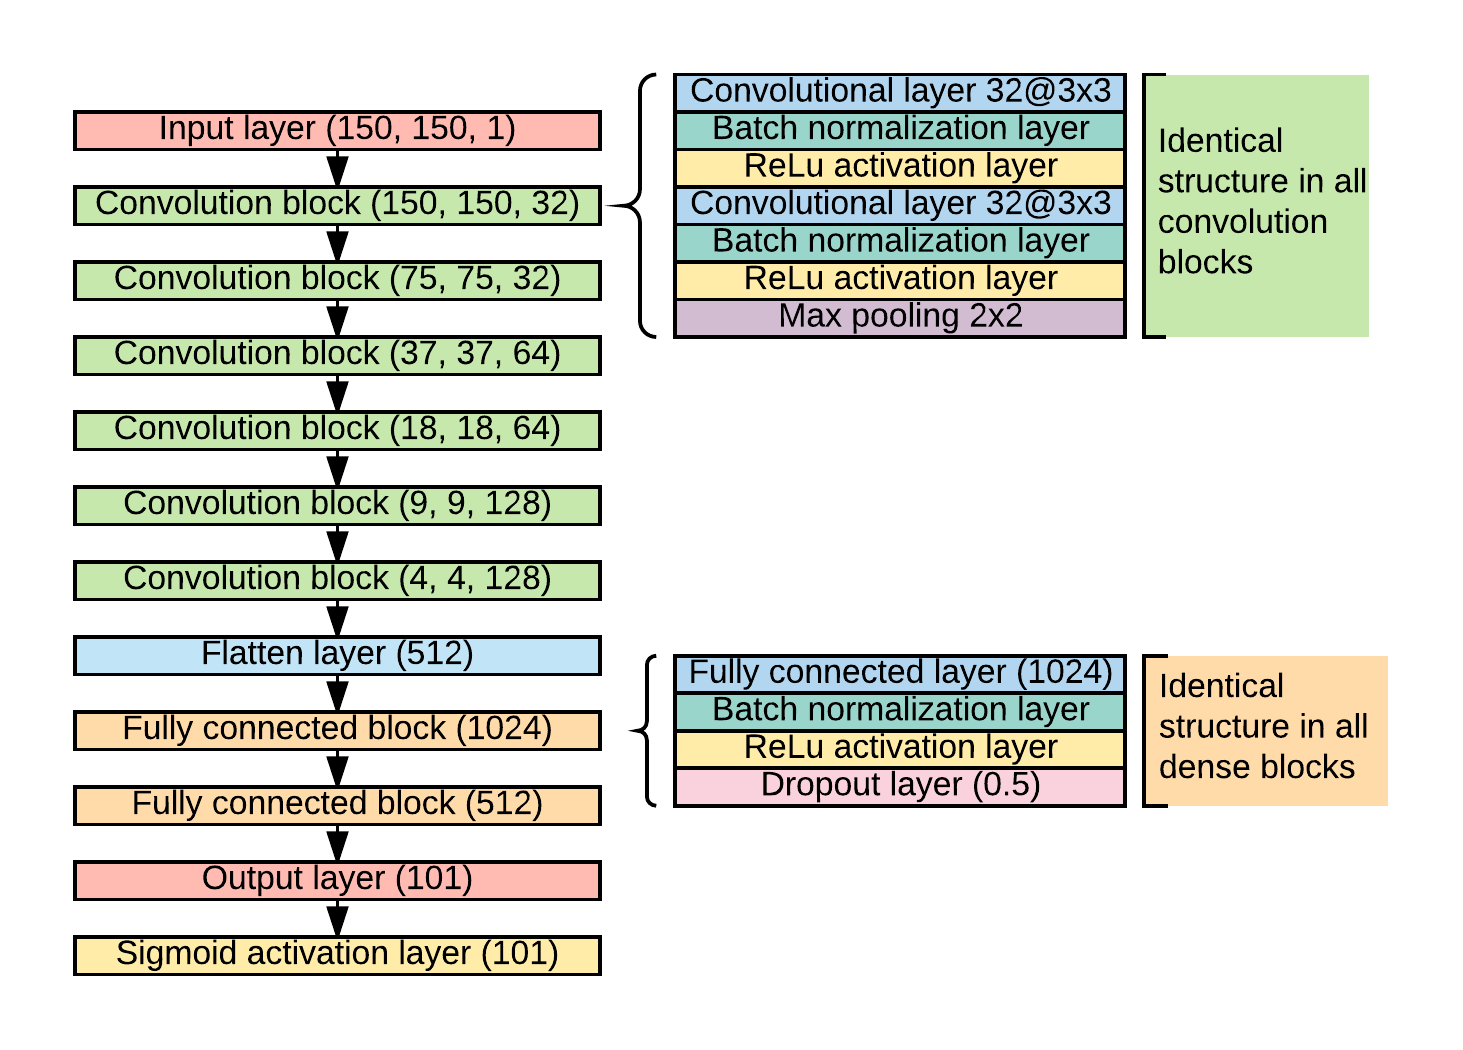
\includegraphics[width=10cm]{cnn_regression}	
\caption{Architecture of the CNN for regression}
\label{fig:cnn_reg}
\end{figure}

To train the model, the Continuous Ranked Probability Score (CRPS) was used as the loss function. For the discrete case it is calculated as follows. \cite{crps}

$$CRPS = \frac{1}{101 * N} \sum\limits_{n=1}^{N} \sum\limits_{k=0}^{101} (P(y \geq k) - H(k - R_n))^2$$

Where $P$ is the predicted distribution, $N$ is the number of observations, $R$ is the actual percentage of bone erosion and $H(x) = \begin{cases}
1 & \text{for $x \geq 0$,}\\
0 & \text{otherwise.}
\end{cases}$ \cite{crps}

It is difficult to visualize CRPS, but the shaded area in \autoref{fig:crps} helps understanding what CRPS does. \cite{crps}

\begin{figure}[ht]
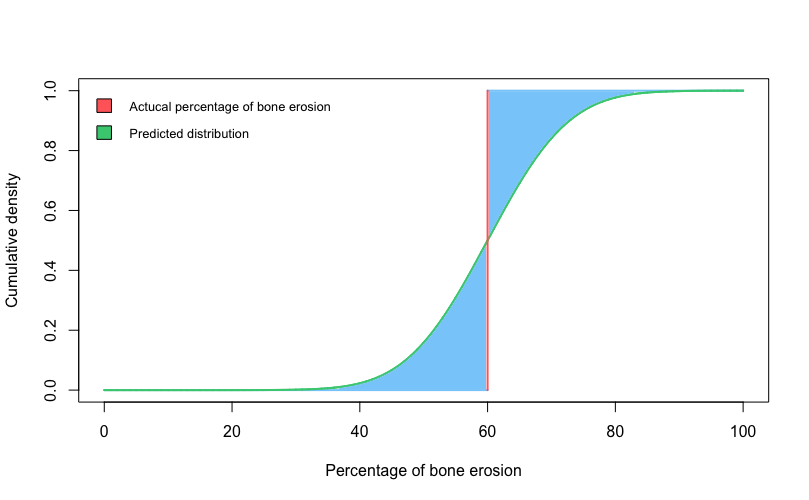
\includegraphics[width=10cm]{crps}	
\caption{CRPS probability score}
\label{fig:crps}
\end{figure}

This model was trained in the same ways as described in \ref{subsubsec:clas} on the original data, oversampled data and with a weighted loss function. This time all three models were trainer for 25 epochs, as they did not start overfitting. \autoref{fig:hexbin} shows the predictions for the test set in all three cases.

\begin{figure}[ht]
\begin{tabular}{ccc}
\subfloat[Original data]{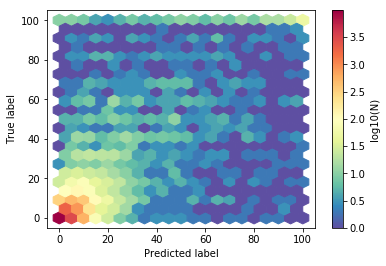
\includegraphics[width = 1.5in]{regression_original}} &
\subfloat[Oversampled]{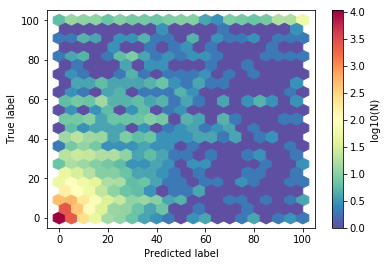
\includegraphics[width = 1.5in]{regression_oversampled}} &
\subfloat[Weights]{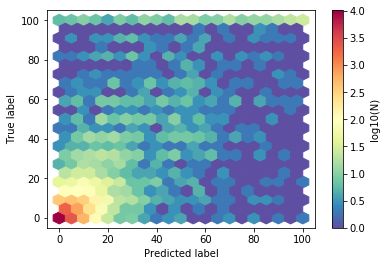
\includegraphics[width = 1.5in]{regression_weights}}
\end{tabular}
\caption{Predictions of the regression models.}
\label{fig:hexbin}
\end{figure}

There is no big visual difference between the three plots. We noticed that the model is not predicting very well for the badly damaged joints with true labels of 100.  

?????????????


When looking at the evaluation metrics in \autoref{tab:metrics_reg}, we can see, that model a) has a smallest mean squared error (mse) as well as the smallest mean absolute error (mae) of the three models. Therefore we decided to use model a) as the base model for regression.

\begin{table}[ht]
\centering
\caption{Evaluation metrics for regression.}
\label{tab:metrics_reg}
\begin{tabular}{@{}llll@{}}
\toprule
                                & a)    & b)    & c)    \\ \midrule
CRPS							& 0.0291 & 0.0304 & 0.0426 \\
Mean squared error (mse)        & 80.884 & 83.017 & 94.488 \\
Mean absolute error (mae)       & 4.046 & 4.072 & 4.057 \\

\bottomrule
\end{tabular}
\end{table}

\subsection{Transfer learning}
\label{subsec:tl}

As Tajbakhsh et al. \cite{tajbakhsh_2017} suggested in their paper, we wanted to try, whether transfer learning could improve our predictions. We decided to use the Inception V3 model \cite{szegedy_2015} which was pre-trained on the Imagenet dataset. We used the pre-trained weights and cut off the output layer. Instead we added two dense layers and an output layer identical to the output layers described in \ref{subsubsec:clas} and \ref{subsubsec:reg} for classification and regression respectively. Since the model is trained on color images, the greyscale images were converted to RGB. The Inception V3 model further requires the input data to be transformed to [-1,1] which was done in an additional pre-processing step.

\begin{figure}[ht]
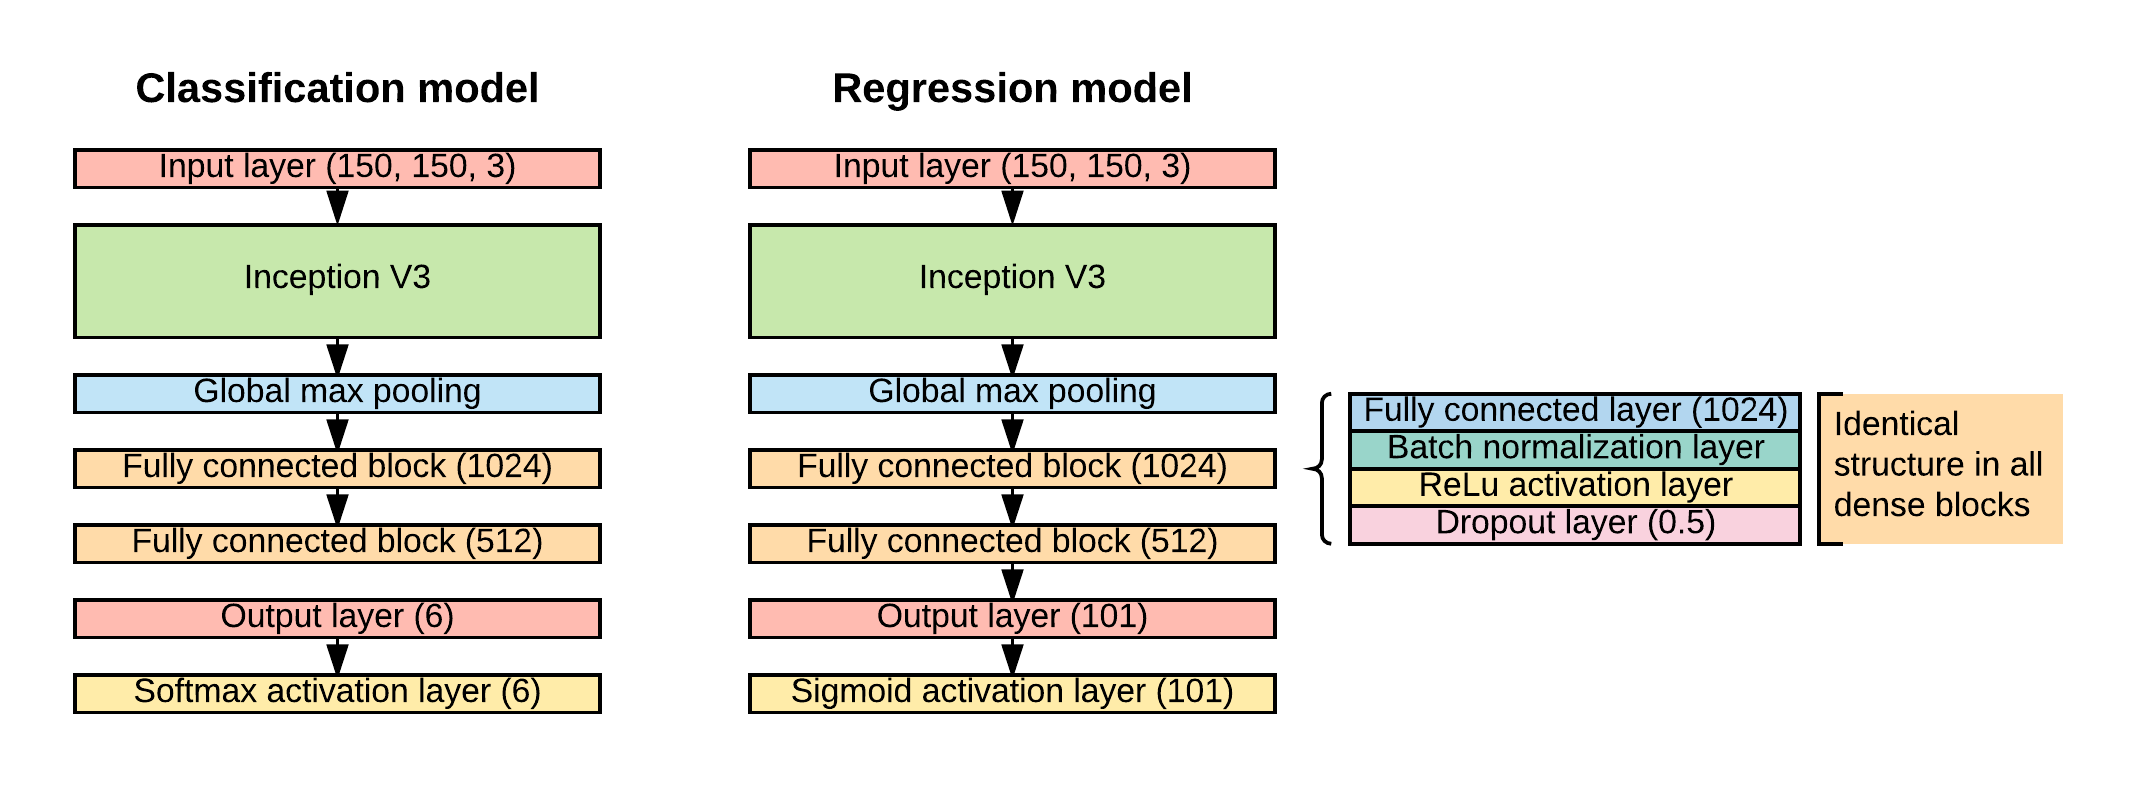
\includegraphics[width=10cm]{transfer_learning}	
\caption{Model architecture for transfer learning}
\label{fig:transfer_learning}
\end{figure}

We then froze all existing weights and only trained the dense layers and the output layer for 25 epochs. Afterwards we repeated the training for all layers for an additional 25 epochs. The predictions for the test set are shown in \autoref{fig:transfer_learning_results}. When comparing the confusion matrix for the classification model with Model c) in \autoref{fig:confusion} we can see that the transfer learning model has higher accuracy for the extreme cases 0, 1 and 5. However, the model seems to perform worse for the Ratingen-scores 2, 3 and 4. The regression model seems to better predict very bad cases with scores of 100. There are still a few outliers, but far fewer than in the base model.

\begin{figure}[ht]
\begin{tabular}{cc}
\subfloat[Classification]{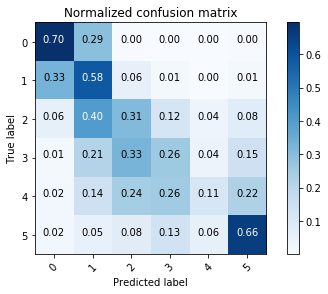
\includegraphics[width = 1.5in]{transfer_learning_classification}} &
\subfloat[Regression]{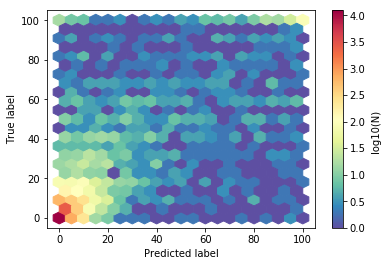
\includegraphics[width = 1.5in]{transfer_learning_regression}}
\end{tabular}
\caption{Predictions of the transfer learning models}
\label{fig:transfer_learning_results}
\end{figure}

\autoref{tab:transfer_learning_metrics} shows the evaluation metrics for the two models. When comparing the metrics to model c) in \autoref{tab:metrics_cla} and model a) in \autoref{tab:metrics_reg} we can see that the classification model has a higher class normalized accuracy but the class normalized accuracy $\pm$ 1 is worse. To compare the accuracies of the two models, Wilson score intervals were used. The Wilson score interval for the normalized accuracy of the base model and the transfer learning model are (0.415, 0.429) and (0.429, 0.443) respectively.

??? +- 1 : base: (0.812, 0.822)
transfer: (0.781, 0.793)


The transfer learning model for classification is not clearly better than the base model. The regression model however is considerably better than the base model with all evaluation metrics showing better results. 

\begin{table}[ht]
\begin{tabular}{cc}
\begin{tabular}{@{}ll@{}}
\toprule
                                & Classification \\ \midrule
Accuracy                        & 0.65           \\
Class normalized accuracy       & 0.436          \\
Class normalized accuracy $\pm$ 1 & 0.787          \\ \bottomrule
\end{tabular}
\quad
\begin{tabular}{@{}ll@{}}
\toprule
        & Regression \\ \midrule
CRPS    & 0.0274          \\
MSE     & 72.768          \\
MAE		& 0.653          \\ \bottomrule
\end{tabular}
\end{tabular}
\caption{Evaluation metrics for the transfer learning models}
\label{tab:transfer_learning_metrics}
\end{table}

\subsection{Analysis of the embeddings}
\label{subsec:embeddings}

To visualize the high-level representations learned by our networks, t-SNE was applied to the outputs of the last hidden layer. Each dot represents an image and the colors represent the true labels of those images. \autoref{fig:tsne_embeddings} shows that both neural networks managed to separate the different scores quite well. However, there are a few images with low scores in the area of the bad scores.

\begin{figure}[ht]
\begin{tabular}{cc}
\subfloat[Classification]{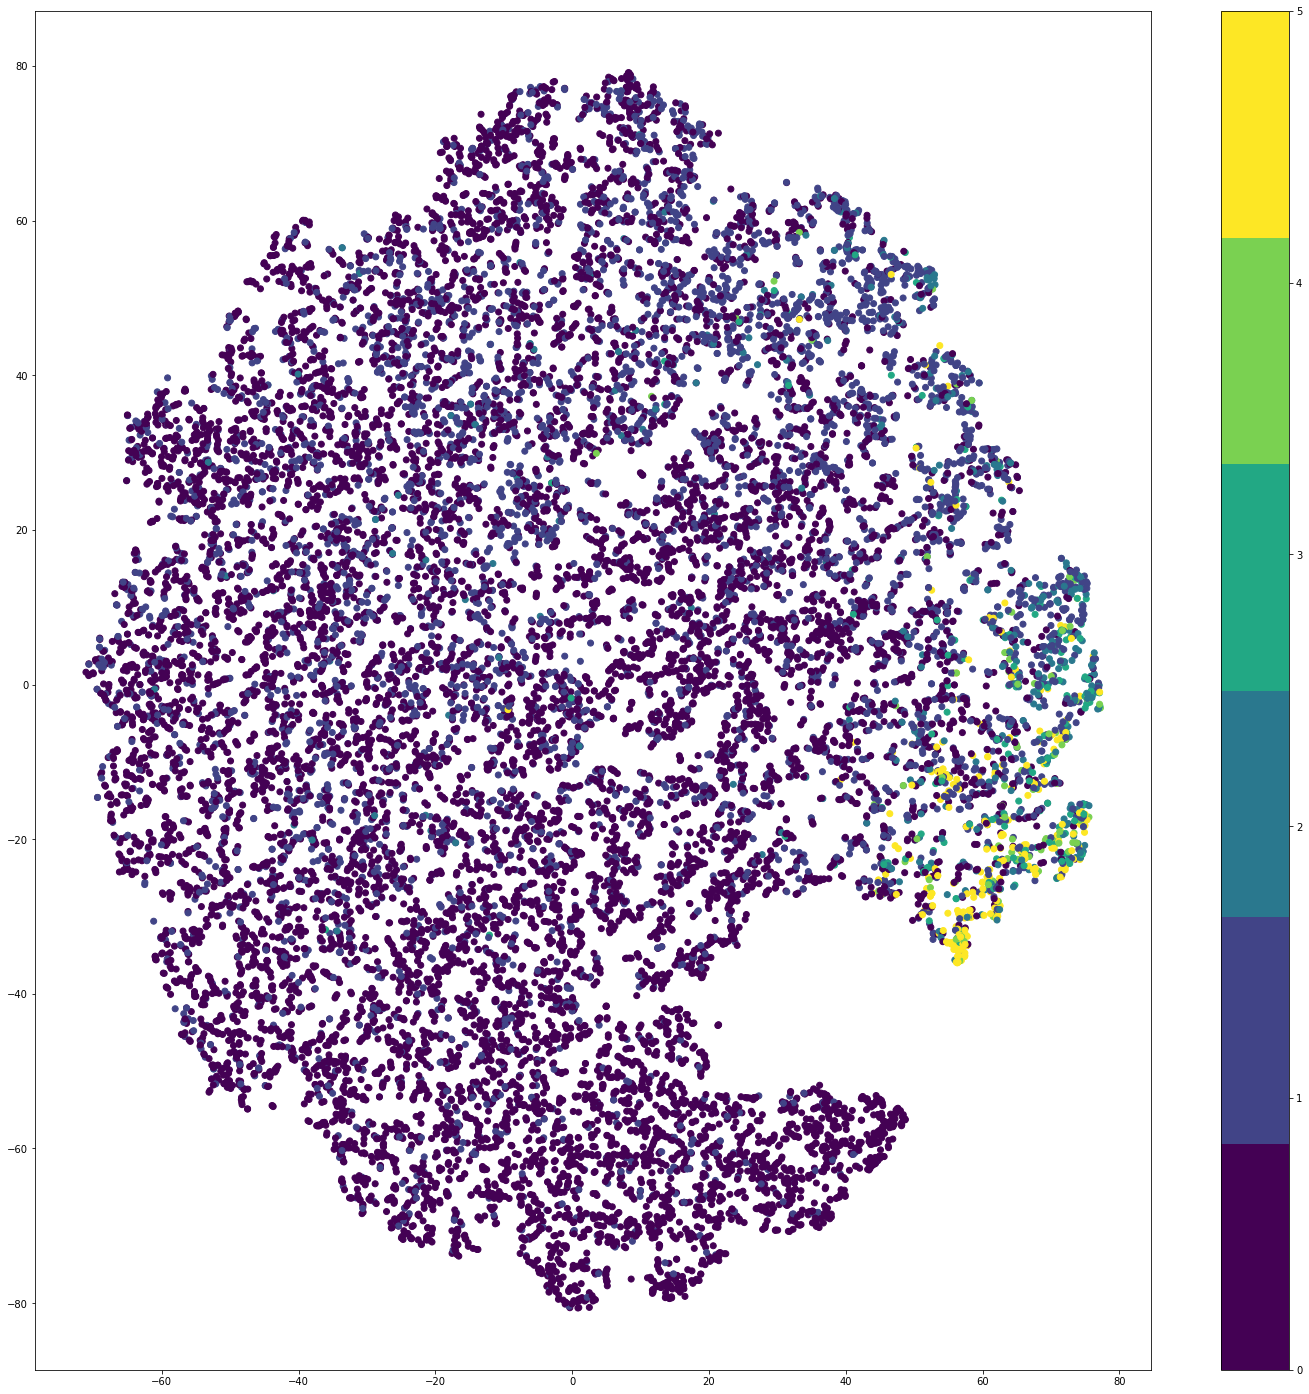
\includegraphics[width = 2.5in]{tsne_classification}} &
\subfloat[Regression]{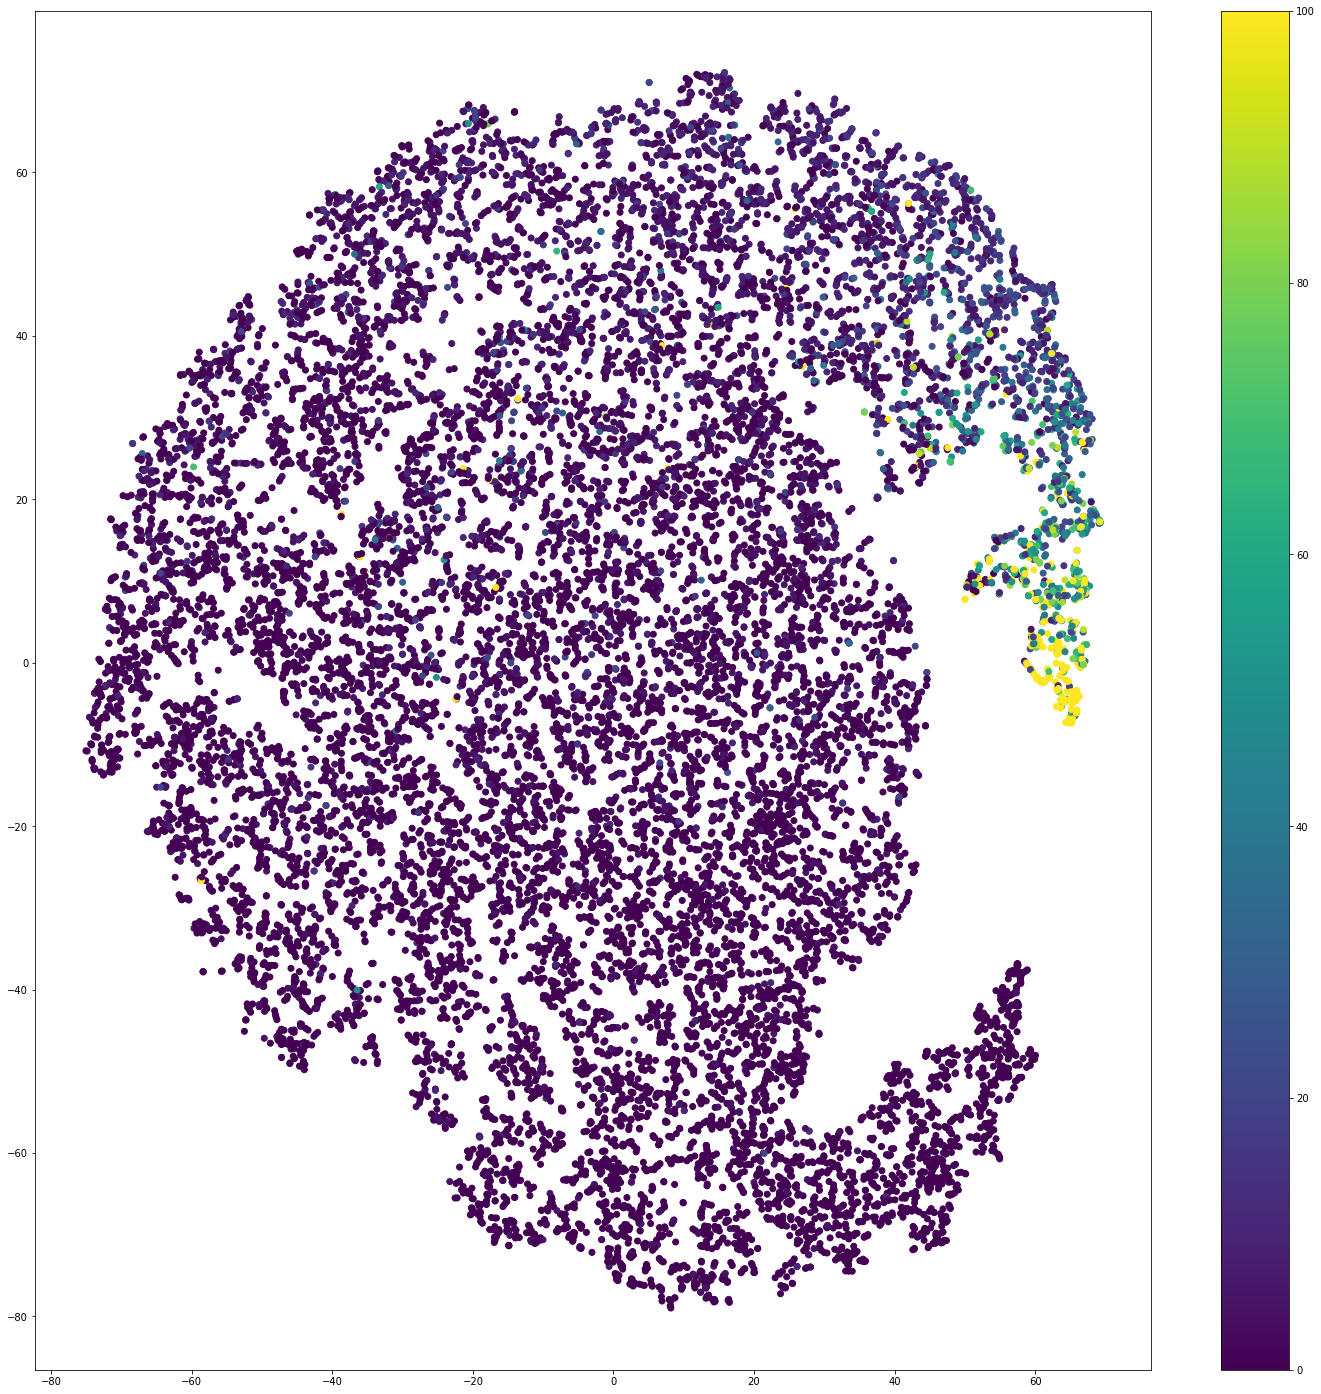
\includegraphics[width = 2.5in]{tsne_regression}}
\end{tabular}
\caption{T-SNE of the embeddings. Each point represents an image (joint) the color represents the bone erosion score.}
\label{fig:tsne_embeddings}
\end{figure}


\subsection{Analysis of correlations between bone erosion and disease activity}
\label{subsec:correlation}

In order to determine wether there is a correlation between the bone erosion scores and the disease activity we compared the Rau-score and the DAS. Both scores are described in \ref{sec:theory}. It is expected that the disease activity score is correlated with the bone erosion score. However, \autoref{fig:correlation} shows that there is only a very weak correlation. Between the two different DAS and the Rau-score.

\begin{figure}[ht]
\begin{tabular}{cc}
\subfloat[BSR]{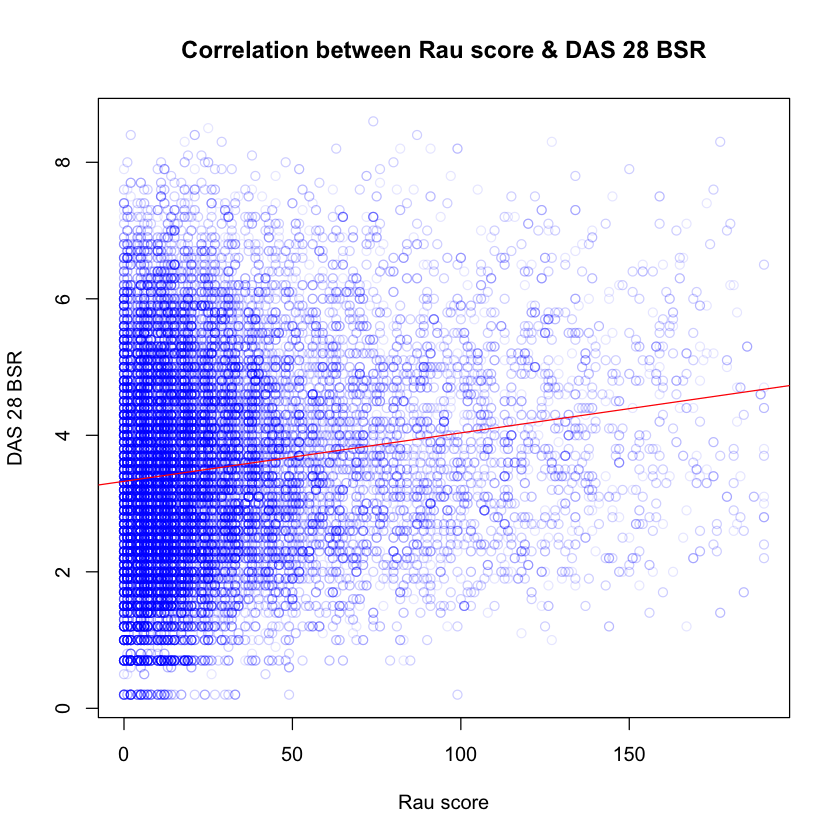
\includegraphics[width = 2.5in]{correlation_bsr}} &
\subfloat[CRP]{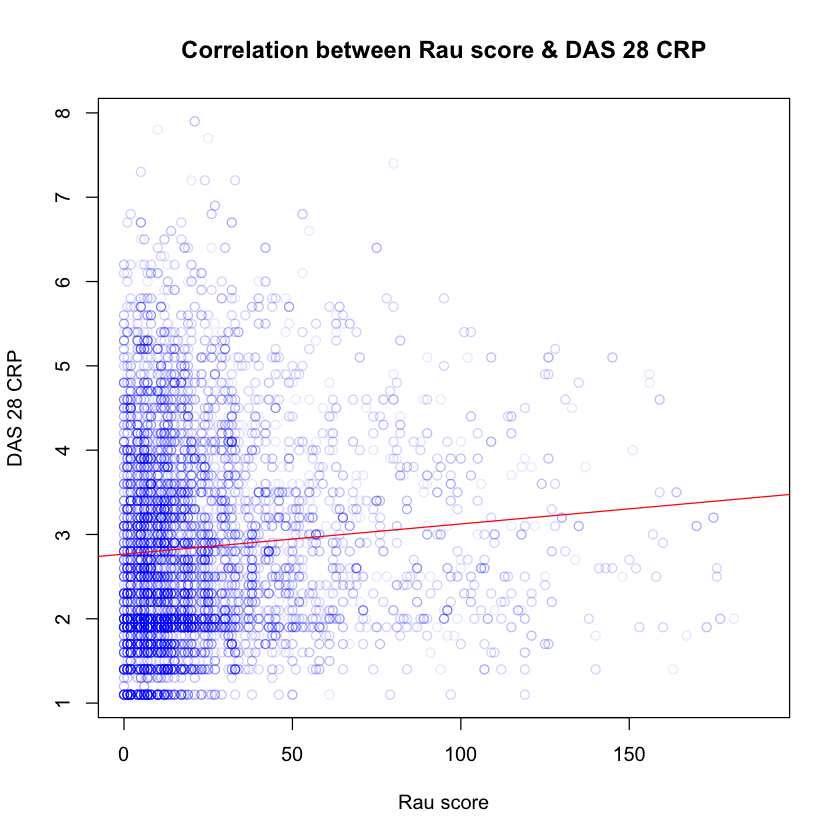
\includegraphics[width = 2.5in]{correlation_crp}}
\end{tabular}
\caption{Scatter plot of DAS compared to Rau-scores}
\label{fig:correlation}
\end{figure}




\newpage
\section{Discussion}
\label{sec:discussion}


\newpage
\section{Conclusion}
\label{sec:conclusion}



\newpage
\printbibliography

\newpage
\listoffigures


\end{document}
